% Graphics for slide 7, in the order the PDF draws them.
\begin{tikzpicture}[remember picture, overlay, x=1bp, y=-1bp,
  shift={(current page.north west)}]
\path[fill=cFFFFFF] (0,0) rectangle (960,540);
\node[anchor=north west, inner sep=0pt] at (56.69,477.21) {
\includegraphics[width=73.42bp, height=37.42bp]{figures/fundamentals-of-hpc/p03-1.png}};
\path[fill=cEE7628,even odd rule] (57.18,55.73) ..controls(57.96,55.73)and(58.6,56.37)..(58.6,57.15) --(58.6,85.5) ..controls(58.6,86.28)and(57.96,86.91)..(57.18,86.91) ..controls(56.4,86.91)and(55.76,86.28)..(55.76,85.5) --(55.76,57.15) ..controls(55.76,56.37)and(56.4,55.73)..(57.18,55.73);
\node[anchor=north west, inner sep=0pt] at (316.24,57.33) {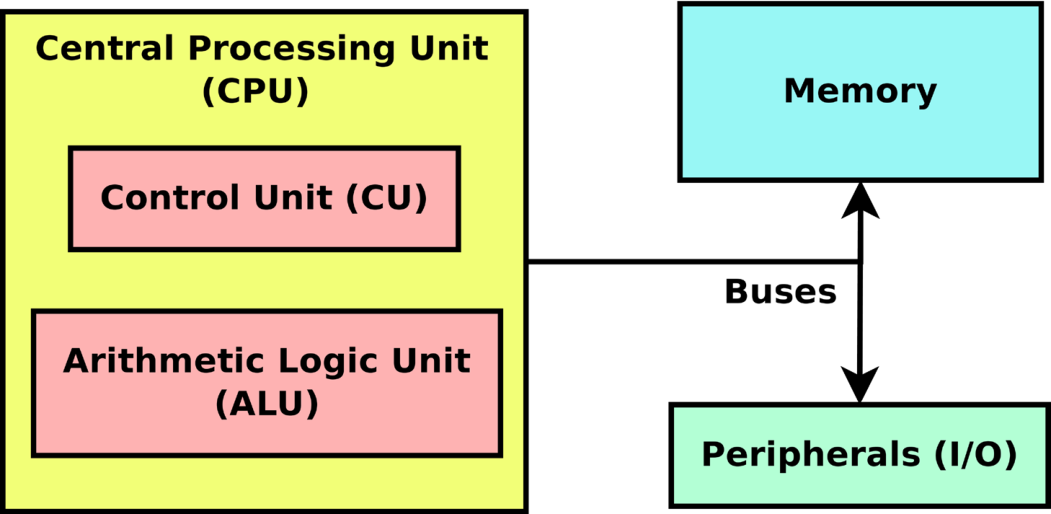
\includegraphics[width=349.84bp, height=171.17bp]{figures/fundamentals-of-hpc/p07-2.png}};
\node[anchor=north west, inner sep=0pt] at (719.46,338.86) {
\includegraphics[width=195.12bp, height=159.22bp]{figures/fundamentals-of-hpc/p07-3.jpg}};
\node[anchor=north west, inner sep=0pt] at (513.7,338.91) {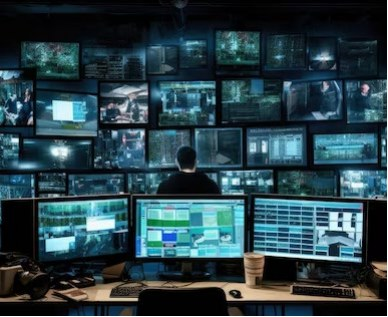
\includegraphics[width=195.51bp, height=159.64bp]{figures/fundamentals-of-hpc/p07-4.jpg}};
\node[anchor=north west, inner sep=0pt] at (719.46,176.58) {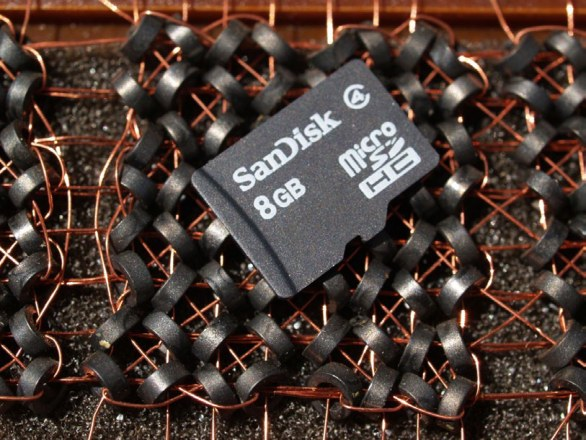
\includegraphics[width=195.1bp, height=146.33bp]{figures/fundamentals-of-hpc/p07-5.jpg}};
\node[anchor=north west, inner sep=0pt] at (55.76,249.62) {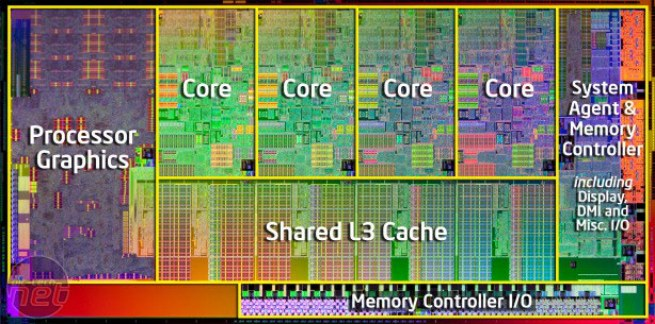
\includegraphics[width=435.62bp, height=215.68bp]{figures/fundamentals-of-hpc/p07-6.jpg}};
\node[anchor=north west, inner sep=0pt] at (55.76,126.41) {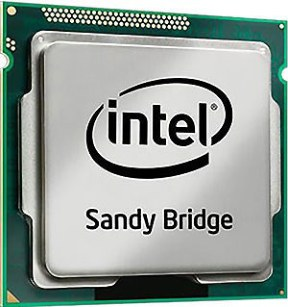
\includegraphics[width=95.89bp, height=101.96bp]{figures/fundamentals-of-hpc/p07-7.jpg}};
\path[draw=cF6DA44,line width=1.5bp] (273.57,249.62) --(314.39,147.56);
\path[fill=cF6DA44,even odd rule] (316.8,149.61) --(316.24,142.92) --(311.23,147.38) --(316.8,149.61);
\path[draw=cF6DA44,line width=1.5bp] (151.65,175.33) --(311.41,132.37);
\path[fill=cF6DA44,even odd rule] (311.23,135.52) --(316.24,131.07) --(309.67,129.73) --(311.23,135.52);
\path[draw=c177ABF,line width=1.5bp] (719.46,176.58) --(669.59,125.73);
\path[fill=c177ABF,even odd rule] (668.14,128.54) --(666.09,122.16) --(672.43,124.34) --(668.14,128.54);
\path[draw=c2CA055,line width=1.5bp] (611.23,338.91) --(603.86,233.5);
\path[fill=c2CA055,even odd rule] (600.94,234.7) --(603.51,228.51) --(606.92,234.28) --(600.94,234.7);
\path[draw=c2CA055,line width=1.5bp] (719.46,338.91) --(642.5,232.56);
\path[fill=c2CA055,even odd rule] (640.65,235.13) --(639.57,228.51) --(645.51,231.61) --(640.65,235.13);
\node[anchor=north west, inner sep=0pt] at (719.46,30.5) {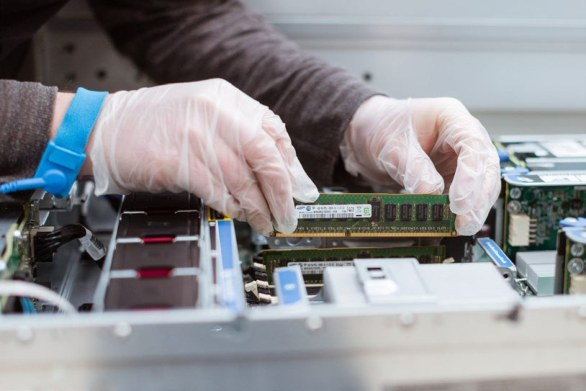
\includegraphics[width=195.18bp, height=130.16bp]{figures/fundamentals-of-hpc/p07-8.jpg}};
\path[draw=c177ABF,line width=1.5bp] (719.46,95.54) --(671.05,89.72);
\path[fill=c177ABF,even odd rule] (671.68,92.82) --(666.09,89.13) --(672.4,86.86) --(671.68,92.82);
\end{tikzpicture}
